
\typeout{************************************************}
\typeout{Chapter 5 Questions Concerning Power Series}
\typeout{************************************************}
%
\begin{chapterptx}{Questions Concerning Power Series}{}{Questions Concerning Power Series}{}{}{x:chapter:PowerSeriesQuestions}
	%
	%
	\typeout{************************************************}
	\typeout{Section 5.1 Taylor's Formula}
	\typeout{************************************************}
	%
	\begin{sectionptx}{Taylor's Formula}{}{Taylor's Formula}{}{}{x:section:PowerSeriesQuestions-TaylorsFormula}
		As we saw in the previous chapter, representing functions as power series was a fruitful strategy for mathematicans in the eighteenth century (as it still is). Differentiating and integrating power series term by term was relatively easy, \emph{seemed} to work, and led to many applications. Furthermore, power series representations for all of the elementary functions could be obtained if one was clever enough.%
		\par
		However, cleverness is an unreliable tool. Is there some systematic way to find a power series for a given function? To be sure, there were nagging questions: If we can find a power series, how do we know that the series we've created represents the function we started with? Even worse, is it possible for a function to have more than one power series representation centered at a given value \(a?\) This uniqueness issue is addressed by the following theorem.%
		\begin{theorem}{}{}{x:theorem:TaylorSeriesThm}%
			\index{Taylor's Formula} If \(f(x)=\sum_{n=0}^\infty a_n(x-a)^n\), then \(a_n=\frac{f^{(n)}(a)}{n!}\), where \(f^{(n)}(a)\) represents the \(n^{th}\) derivative of \(f\) evaluated at \(a\).%
		\end{theorem}
		A few comments about \hyperref[x:theorem:TaylorSeriesThm]{Theorem~{\xreffont\ref{x:theorem:TaylorSeriesThm}}} are in order. Notice that we did \emph{not} start with a function and derive its series representation. Instead we \emph{defined} \(f(x)\) to be the series we wrote down. This assumes that the expression \(\sum_{n=0}^\infty a_n(x-a)^n\) actually has meaning (that it converges). At this point we have every reason to expect that it does, however expectation is not proof so we note that this is an assumption, not an established truth. Similarly, the idea that we can differentiate an infinite polynomial term-by-term as we would a finite polynomial is also assumed. As before, we follow in the footsteps of our 18th century forebears in making these assumptions. For now.%
		\begin{problem}{}{g:problem:idp77}%
			\index{Taylor's Formula} Prove \hyperref[x:theorem:TaylorSeriesThm]{Theorem~{\xreffont\ref{x:theorem:TaylorSeriesThm}}}.%
			\par\smallskip%
			\noindent\textbf{\blocktitlefont Hint}.\hypertarget{g:hint:idp78}{}\quad{}\(f(a)=a_0+a_1(a-a)+a_2(a-a)^2+\cdots=a_0\). Differentiate to obtain the other terms.%
		\end{problem}
		From \hyperref[x:theorem:TaylorSeriesThm]{Theorem~{\xreffont\ref{x:theorem:TaylorSeriesThm}}} we see that if we do start with the function \(f(x)\) then no matter how we obtain its power series, the result will always be the same. The series%
		\begin{equation*}
			\sum_{n=0}^\infty\frac{f^{(n)}(a)}{n!}(x-a)^n=f(a)+f^\prime(a)(x-a)+\frac{f^{\prime\prime}(a)}{2!}(x-a)^2+\frac{f^{\prime\prime\prime}(a)}{3!}(x-a)^3+\cdots
		\end{equation*}
		%
		\begin{figureptx}{\href{https://mathshistory.st-andrews.ac.uk/Biographies/Taylor/}{Brook Taylor}\protect\footnotemark{}}{g:figure:idp79}{}%
			\index{Taylor, Brook!portrait of}%
			\begin{image}{0.325}{0.35}{0.325}%
				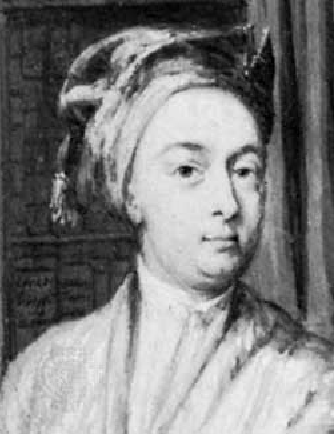
\includegraphics[width=\linewidth]{external/images/Taylor.png}
			\end{image}%
			\tcblower
		\end{figureptx}%
		\footnotetext[11]{\nolinkurl{mathshistory.st-andrews.ac.uk/Biographies/Taylor/}\label{g:fn:idp80}}%
		is called the \emph{\alert{Taylor series} for \(f\) expanded about (centered at) \(a\)}. Although this systematic ``machine'' for obtaining power series for a function seems to have been known to a number of mathematicians in the early 1700's, Brook Taylor \index{Taylor, Brook} was the first to publish this result in his \textit{Methodus Incrementorum} (1715). The special case when \(a=0\) was included by Colin Maclaurin \index{Maclaurin, Colin} in his \emph{Treatise of Fluxions} (1742). Thus when \(a=0\), the series \(\sum_{n=0}^\infty\frac{f^{(n)}(0)}{n!}x^n\) is often called the \emph{Maclaurin Series for \(f\)}.%
		\par
		The ``prime notation'' for the derivative was not used by Taylor, \index{Taylor, Brook} Maclaurin or their contemporaries. It was introduced by Joseph Louis Lagrange \index{Lagrange, Joseph-Louis} in his 1779 work \textit{Théorie des Fonctions Analytiques}. In that work, Lagrange sought to get rid of Leibniz's infinitesimals\index{Leibniz, Gottfried Wilhelm} and base calculus on the power series idea. His idea was that by representing every function as a power series, calculus could be done ``algebraically'' by manipulating power series and examining various aspects of the series representation instead of appealing to the ``controversial'' notion of infinitesimals. He implicitly assumed that every continuous function could be replaced with its power series representation.%
		\par
		That is, he wanted to think of the Taylor series as a ``great big polynomial,'' because polynomials are easy to work with. It was a very simple, yet exceedingly clever and far-reaching idea. Since \(e^x = 1 +x +x^2/2 +\ldots\), for example, why not just define the exponential to be the series and work with the series. After all, the series is just a very long polynomial.%
		\par
		This idea did not come out of nowhere. Leonhard Euler \index{Euler, Leonhard} had put exactly that idea to work to solve many problems throughout the 18th century. Some of his solutions are still quite breath-taking when you first see them~\hyperlink{x:biblio:sandifer07__early_mathem_leonar_euler}{[{\xreffont 14}]}.%
		\par
		Taking his cue from the Taylor series%
		\begin{equation*}
			f(x) = \sum_{n=0}^\infty\frac{f^{(n)}(a)}{n!}(x-a)^n
		\end{equation*}
		%
		\begin{figureptx}{\href{https://mathshistory.st-andrews.ac.uk/Biographies/Lagrange/}{Joseph-Louis Lagrange}\protect\footnotemark{}}{g:figure:idp81}{}%
			\index{Lagrange, Joseph-Louis!portrait of}%
			\begin{image}{0.325}{0.35}{0.325}%
				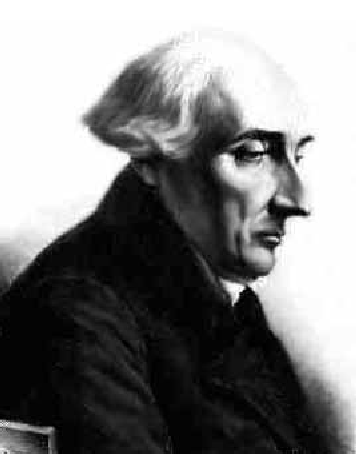
\includegraphics[width=\linewidth]{external/images/Lagrange.png}
			\end{image}%
			\tcblower
		\end{figureptx}%
		\footnotetext[12]{\nolinkurl{mathshistory.st-andrews.ac.uk/Biographies/Lagrange/}\label{g:fn:idp82}}%
		Lagrange observed that the coefficient of \((x-a)^n\) provides the derivative of \(f\) at \(a\) (divided by \(n!\)). Modifying the formula above to suit his purpose, Lagrange supposed that every differentiable function could be represented as%
		\begin{equation*}
			f(x) = \sum_{n=0}^\infty g_n(a)(x-a)^n\text{.}
		\end{equation*}
		%
		\par
		If we regard the parameter \(a\) as a variable then \(g_1\) is the derivative of \(f\), \(g_2=2f^{\prime\prime}\) and generally%
		\begin{equation*}
			g_n=n!f^{(n)}\text{.}
		\end{equation*}
		%
		\par
		Lagrange dubbed his function \(g_1\) the \textit{``fonction dérivée''} from which we get the modern name ``derivative.''%
		\par
		All in all, this was a very clever and insightful idea whose only real flaw is that its fundamental assumption is not true. It turns out that not every differentiable function can be represented as a Taylor series. This was demonstrated very dramatically by Augustin Cauchy's \index{Cauchy, Augustin} famous counter-example%
		\begin{equation}
			f(x) = \begin{cases} e^{-\frac{1}{x^2}}\amp  x\ne0\\ 0 \amp x=0 \end{cases}\text{.}\label{x:men:eq_CauchyCounterEx}
		\end{equation}
		%
		\par
		This function is actually infinitely differentiable everywhere but its Maclaurin series (that is, a Taylor series with \(a=0\)) does not converge to \(f\) because all of its derivatives at the origin are equal to zero: \(f^{(n)}(0) = 0, \forall n\in\NN\).%
		\par
		Computing these derivatives using the definition you learned in calculus is not conceptually difficult but the formulas involved do become complicated rather quickly. Some care must be taken to avoid error.%
		\par
		To begin with, let's compute a few derivatives when \(x \neq 0\).%
		\begin{align*}
			f^{(0)}(x) \amp = e^{x^{-2}}\\
			f^{(1)}(x) \amp = 2x^{-3}e^{-x^{-2}}\\
			f^{(2)}(x) \amp = \left(4x^{-6}-6x^{-4}\right)e^{-x^{-2}}\text{.}
		\end{align*}
		%
		\par
		As you can see the calculations are already getting a little complicated and we've only taken the second derivative. To streamline things a bit we take \(y= x^{-1}\), and define \(p_2(x) = 4x^6-6x^4\) so that%
		\begin{equation*}
			f^{(2)}(x) = p_2(x^{-1})e^{-x^{-2}} = p_2(y)e^{-y^2}\text{.}
		\end{equation*}
		%
		\begin{problem}{Cauchy's Counterexample, Part 1.}{g:problem:idp83}%
			\begin{enumerate}[font=\bfseries,label=(\alph*),ref=\alph*]
				\item{}Adopting the notation \(y=x^{-1}\) and \(f^{(n)}(x) =p_n(y)e^{-y^2}\), find \(p_{n+1}(y)\) in terms of \(p_{n}(y)\). [Note: Don't forget that you are differentiating with respect to \(x\), not \(y\).]%
				\item{}Use induction on \(n\) to show that \(p_n(y)\) is a polynomial for all \(n\in\NN\).%
			\end{enumerate}
		\end{problem}
		Unfortunately everything we've done so far only gives us the derivatives we need when \(x\) is \emph{not} zero, and we need the derivatives when \(x\) \emph{is} zero. To find these we need to get back to very basic ideas.%
		\par
		Let's assume for the moment that we know that \(f^{(n)}(0)=0\) and recall that%
		\begin{align*}
			f^{(n+1)}(0) \amp = \limit{x}{0}{\frac{f^{(n)}(x)-f^{(n)}(0)}{x-0}}\\
			f^{(n+1)}(0) \amp = \limit{x}{0}{x^{-1}p_n(x^{-1})e^{-x^{-2}}}\\
			f^{(n+1)}(0) \amp = \limit{y}{\pm\infty}{\frac{yp_n(y)}{e^{y^2}}}\text{.}
		\end{align*}
		%
		\par
		We can close the deal with the following problem.%
		\begin{problem}{Cauchy's Counterexample, Part 2.}{g:problem:idp84}%
			\begin{enumerate}[font=\bfseries,label=(\alph*),ref=\alph*]
				\item{}Let \(m\) be a nonnegative integer. Show that \(\limit{y}{\pm\infty}{\frac{y^m}{e^{y^2}}}=0\).%
				\par\smallskip%
				\noindent\textbf{\blocktitlefont Hint}.\hypertarget{g:hint:idp85}{}\quad{}Induction and a dash of L'Hôpital's rule should do the trick.%
				\item{}Prove that \(\limit{y}{\pm\infty}{\frac{q(y)}{e^{y^2}}}=0\) for any polynomial \(q\).%
				\item{}Let \(f(x)\) be as in \hyperref[x:men:eq_CauchyCounterEx]{equation~({\xreffont\ref{x:men:eq_CauchyCounterEx}})} and show that for every nonnegative integer \(n\), \(f^{(n)}(0)=0\).%
			\end{enumerate}
		\end{problem}
		This example showed that while it was fruitful to exploit Taylor series representations of various functions, basing the foundations of calculus on power series was not a sound idea.%
		\par
		While Lagrange's \index{Lagrange, Joseph-Louis} approach wasn't totally successful, it was a major step away from infinitesimals and toward the modern approach. We still use aspects of it today. For instance we still use his prime notation (\(f^\prime\)) to denote the derivative.%
		\par
		Turning Lagrange's idea on its head it is clear that if we know how to compute derivatives, we can use this machine to obtain a power series when we are not ``clever enough'' to obtain the series in other (typically shorter) ways. For example, consider Newton's binomial series when \(\alpha=\frac{1}{2}\). Originally, we obtained this series by extending the binomial theorem to non-integer exponents. Taylor's formula provides a more systematic way to obtain this series:%
		\begin{align*}
			f(x)\amp =(1+x)^{\frac{1}{2}};\amp f(0)\amp =1\\
			f^\prime(x)\amp =\frac{1}{2}(1+x)^{\frac{1}{2}-1};\amp  f^\prime(0)\amp =\frac{1}{2}\\
			f^{\prime\prime}(x)\amp =\frac{1}{2}\left(\frac{1}{2}-1\right)(1+x)^{\frac{1}{2}-2}\amp f^{\prime\prime}(0)\amp =\frac{1}{2}\left(\frac{1}{2}-1\right)
		\end{align*}
		and in general since%
		\begin{align*}
			f^{(n)}(x)\amp =\frac{1}{2}\left(\frac{1}{2}-1\right)\cdots\left(\frac{1}{2}-(n-1)\right)(1+x)^{\frac{1}{2}-n}\\
			\intertext{we have}
			f^{(n)}(0)\amp =\frac{1}{2}\left(\frac{1}{2}-1\right)\cdots\left(\frac{1}{2}-(n-1)\right)\text{.}
		\end{align*}
		%
		\par
		Using Taylor's formula we obtain the series%
		\begin{equation*}
			\sum_{n=0}^\infty\frac{f^{(n)}(0)}{n!}x^n = 1+\sum_{n=1}^\infty\frac{\frac{1}{2}\left(\frac{1}{2}-1\right)\cdots\left( \frac{1}{2}-(n-1)\right)}{n!}x^n= 1+\sum_{n=1}^\infty\frac{\prod_{j=0}^{n-1}\left(\frac{1}{2}-j\right)}{n!}x^n
		\end{equation*}
		which agrees with \hyperref[x:men:eq_BinomialSeries]{equation~({\xreffont\ref{x:men:eq_BinomialSeries}})} in the previous chapter.%
		\begin{problem}{}{g:problem:idp86}%
			\index{Taylor's Formula!use to obtain the general binomial series} Use Taylor's formula to obtain the general binomial series%
			\begin{equation*}
				(1+x)^\alpha=1+\sum_{n=1}^\infty\frac{\prod_{j=0}^{n-1}\left(\alpha-j\right)}{n!}x^n.{}
			\end{equation*}
			%
		\end{problem}
		\begin{problem}{}{g:problem:idp87}%
			\index{\(e^x\)!Taylor's series for}\index{series!Taylor's series!expansion of \(e^x, \sin x\), and \(\cos x\)}\index{\(\sin x\)!Taylor's series for}\index{\(\cos x\)!Taylor's series for} Use Taylor's formula to obtain the Taylor series for the functions \(e^x\), sin \(x\), and cos \(x\) expanded about \(a\).%
		\end{problem}
		As you can see, Taylor's ``machine'' will produce the power series for a function (if it has one), but is tedious to perform. We will find, generally, that this tediousness can be an obstacle to understanding. In many cases it will be better to be clever if we can. This is usually shorter. However, it is comforting to have Taylor's formula available as a last resort.%
		\par
		The existence of a Taylor series is addressed (to some degree) by the following.%
		\begin{theorem}{}{}{x:theorem:TaylorsTheorem}%
			\index{Taylor's Theorem} If \(f^\prime,\,f^{\prime\prime},\,\ldots,\,f^{(n+1)}\) are all continuous on an interval containing \(a\) and \(x\), then%
			\begin{align*}
				f(x)=f(a)+\frac{f^{\prime}(a)}{1!}(x-a)+\frac{f^{\prime \prime}(a)}{2!}(x-a)^2\amp +\cdots+\frac{f^{(n)}(a)}{n!}(x-a)^n\\
				\amp + \frac{1}{n!}\int_{t=a}^xf^{(n+1)}(t)(x-t)^n\dx{t}\text{.}
			\end{align*}
			%
		\end{theorem}
		Before we address the proof, notice that the \(n\)-th degree polynomial%
		\begin{equation*}
			f(a)+\frac{f^{\,\prime}(a)}{1!}(x-a)+\frac{f^{\,\prime\prime}(a)}{2!}(x-a)^2+\cdots+\frac{f^{(n)}(a)}{n!}(x-a)^n
		\end{equation*}
		resembles the Taylor series and, in fact, is called the \emph{\(n\)-th degree Taylor polynomial of \(f\) about \(a\).} \hyperref[x:theorem:TaylorsTheorem]{Theorem~{\xreffont\ref{x:theorem:TaylorsTheorem}}} says that a function can be written as the sum of this polynomial and a specific integral which we will analyze in the next chapter. We will get the proof started and leave the formal induction proof as an exercise.%
		\par
		Notice that the case when \(n=0\) is really a restatement of the Fundamental Theorem of Calculus. Specifically, the FTC says \(\int_{t=a}^xf^\prime(t)\dx{ t}=f(x)-f(a)\) which we can rewrite as%
		\begin{equation*}
			f(x)=f(a)+\frac{1}{0!}\int_{t=a}^xf^\prime(t)(x-t)^0\dx{ t}
		\end{equation*}
		to provide the anchor step for our induction.%
		\par
		To derive the case where \(n=1\), we use integration by parts. If we let%
		\begin{align*}
			u\amp =f^\prime(t)\amp  d v\amp =(x-t)^0d t\\
			d u\amp =f^{\prime\prime}(t)d t\amp  v\amp =-\frac{1}{1}(x-t)^1
		\end{align*}
		we obtain%
		\begin{align*}
			f(x)\amp =f(a)+\frac{1}{0!}\left(-\frac{1}{1}f^\prime(t)(x-t)^1|_{t=a}^{^x}+\frac{1}{1} \int_{t=a}^xf^{\prime\prime}(t)(x-t)^1\dx{ t}\right)\\
			\amp =f(a)+\frac{1}{0!}\left(-\frac{1}{1}f^\prime(x)(x-x)^1+ \frac{1}{1}f^\prime(a)(x-a)^1+\frac{1}{1}\int_{t=a}^xf^{\prime\prime}(t)(x-t)^1\dx{ t}\right)\\
			\amp =f(a)+\frac{1}{1!}f^\prime(a)\left(x-a\right)^1 + \frac{1}{1!}\int_{t=a}^xf^{\prime\prime}(t)(x-t)^1\dx{ t}\text{.}
		\end{align*}
		%
		\begin{problem}{}{g:problem:idp88}%
			\index{Taylor's Theorem} Provide a formal induction proof for \hyperref[x:theorem:TaylorsTheorem]{Theorem~{\xreffont\ref{x:theorem:TaylorsTheorem}}}.%
		\end{problem}
	\end{sectionptx}
	%
	%
	\typeout{************************************************}
	\typeout{Section 5.2 Series Anomalies}
	\typeout{************************************************}
	%
	\begin{sectionptx}{Series Anomalies}{}{Series Anomalies}{}{}{x:section:PowerSeriesQuestions-SeriesAnomalies}
		Up to this point, we have been somewhat frivolous in our approach to series. This approach mirrors eighteenth century mathematicians who ingeniously exploited calculus and series to provide mathematical and physical results which were virtually unobtainable before. Mathematicans were eager to push these techniques as far as they could to obtain their results and they often showed good intuition regarding what was mathematically acceptable and what was not. However, as the envelope was pushed, questions about the validity of the methods surfaced.%
		\par
		As an illustration consider the series expansion%
		\begin{equation*}
			\frac{1}{1+x}=1-x+x^2-x^3+\cdots\text{.}
		\end{equation*}
		%
		\par
		If we substitute \(x=1\) into this equation, we obtain%
		\begin{equation*}
			\frac{1}{2}=1-1+1-1+\cdots\text{.}
		\end{equation*}
		%
		\par
		If we group the terms as follows \((1-1)+(1-1)+\cdots\), the series would equal \(0\). A regrouping of \(1+(-1+1)+(-1+1)+\cdots\) provides an answer of \(1\). This violation of the associative law of addition did not escape the mathematicians of the 1700's. In his 1760 paper \emph{On Divergent Series} Euler \index{Euler, Leonhard} said:%
		\begin{quote}%
			Notable enough, however are the controversies over the series \(1-1+1-1+etc\), \index{Leibniz, Gottfried Wilhelm} whose sum was given by Leibniz as \(\frac{1}{2}\), although others disagree .~.~. Understanding of this question is to be sought in the word ``sum;'' this idea, if thus conceived - namely, the sum of a series is said to be that quantity to which it is brought closer as more terms of a series are taken - has relevance only for the convergent series, and we should in general give up this idea of sum for divergent series. On the other hand, as series in analysis arise from the expansion of fractions or irrational quantities or even of transcendentals, it will, in turn, be permissible in calculation to substitute in place of such series that quantity out of whose development it is produced.%
		\end{quote}
		Even with this formal approach to series, an interesting question arises. The series for the antiderivative of \(\frac{1}{1+x}\) \emph{does} converge for \(x=1\) while this one does not. Specifically, taking the antiderivative of the above series, we obtain%
		\begin{equation*}
			\ln(1+x)=x-\frac{1}{2}x^2+\frac{1}{3}x^3-\cdots\text{.}
		\end{equation*}
		%
		\par
		If we substitute \(x=1\) into this series, we obtain \(\ln 2=1-\frac{1}{2}+\frac{1}{3}-\cdots\). It is not hard to see that such an alternating series converges. The following picture shows why. In this diagram, \(S_n\) denotes the partial sum \(1-\frac{1}{2}+\frac{1}{3}-\cdots+\frac{(-1)^{n+1}}{n}\).%
		\begin{image}{0.05}{0.9}{0.05}%
			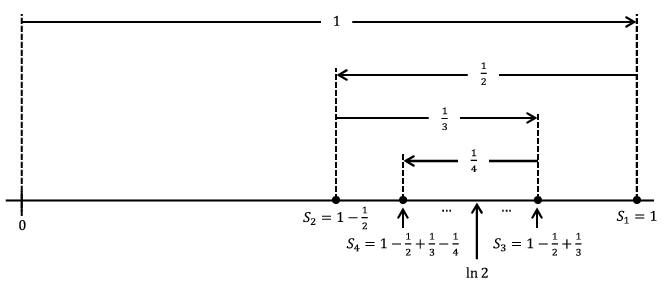
\includegraphics[width=\linewidth]{external/images/AltHarmonic.png}
		\end{image}%
		From the diagram we can see \(S_2\leq S_4\leq S_6\leq\cdots\leq\cdots\leq S_5\leq S_3\leq S_1\) and \(S_{2k+1}-S_{2k}=\frac{1}{2k+1}\). It seems that the sequence of partial sums will converge to whatever is in the ``middle.'' Our diagram indicates that it is ln \(2\) in the middle but actually this is not obvious. Nonetheless it is interesting that one series converges for \(x=1\) but the other does not.%
		\begin{problem}{}{g:problem:idp89}%
			\index{series!Taylor's series!used to approximate \(\ln 2\)} Use the fact that%
			\begin{equation*}
				1-\frac{1}{2}+\frac{1}{3}-\cdots+\frac{(-1)^{2k+1}}{2k}\leq\ln 2\leq 1-\frac{1}{2}+\frac{1}{3}-\cdots+\frac{(-1)^{2k+2}}{2k+1}
			\end{equation*}
			to determine how many terms of the series \(\sum_{n=1}^\infty\frac{(-1)^{n+1}}{n}\) should be added together to approximate \(\ln 2\) to within \(.0001\) without actually computing what \(\ln 2\) is.%
		\end{problem}
		There is an even more perplexing situation brought about by these examples. An infinite sum such as \(1-1+1-1+\cdots\) appears to not satisfy the associative law for addition. While a convergent series such as \(1-\frac{1}{2}+\frac{1}{3}-\cdots\) does satisfy the associative law, it does not satisfy the commutative law. In fact, it does not satisfy it rather spectacularly.%
		\par
		A generalization of the following result was stated and proved by Bernhard Riemann \index{Riemann, Bernhard} in 1854.%
		\begin{theorem}{}{}{x:theorem:thm_rearrangements}%
			\index{series!Alternating Harmonic Series!rearrangements of}%
			Let \(a\) be any real number. There exists a rearrangement of the series \(1-\frac{1}{2}+\frac{1}{3}-\cdots\) which converges to \(a\).%
		\end{theorem}
		This theorem shows that a series is most decidedly \emph{not} a great big sum. It follows that a power series is \emph{not} a great big polynomial.%
		\par
		To set the stage, consider the \emph{harmonic series} \index{series!Harmonic Series}%
		\begin{equation*}
			\sum_{n=1}^\infty\frac{1}{n}=1+\frac{1}{2}+\frac{1}{3}+\cdots\text{.}
		\end{equation*}
		%
		\par
		Even though the individual terms in this series converge to \(0\), the series still diverges (to infinity) as evidenced by the inequality%
		\begin{align*}
			\left(1+\frac{1}{2}\right)\amp +\left(\frac{1}{3}+\frac{1}{4}\right)+\left(\frac{1}{5}+\frac{1}{6}+ \frac{1}{7}+\frac{1}{8}\right)+\left(\frac{1}{9}+\cdots+\frac{1}{16}\right)+\cdots\\
			\amp >\frac{1}{2}+\left(\frac{1}{4}+\frac{1}{4}\right)+\left(\frac{1}{8}+ \frac{1}{8}+\frac{1}{8}+\frac{1}{8}\right)+\left(\frac{1}{16}+\cdots+\frac{1}{16}\right)+\cdots\\
			\amp =\frac{1}{2}+\frac{1}{2}+\frac{1}{2}+\frac{1}{2}+\cdots\\
			\amp =   \infty\text{.}
		\end{align*}
		%
		\par
		Armed with this fact, we can see why \hyperref[x:theorem:thm_rearrangements]{Theorem~{\xreffont\ref{x:theorem:thm_rearrangements}}} is true. First note that%
		\begin{equation*}
			-\frac{1}{2}-\frac{1}{4}-\frac{1}{6}-\cdots=-\frac{1}{2}(1+\frac{1}{2}+ \frac{1}{3}+\cdots)=-\infty
		\end{equation*}
		and%
		\begin{equation*}
			1+\frac{1}{3}+\frac{1}{5}+\cdots\geq\frac{1}{2}+\frac{1}{4}+\frac{1}{6}+\ldots= \infty\text{.}
		\end{equation*}
		%
		\par
		This says that if we add enough terms of \(-\frac{1}{2}-\frac{1}{4}-\frac{1}{6}-\cdots\) we can make such a sum as small as we wish and if we add enough terms of \(1+\frac{1}{3}+\frac{1}{5}+\cdots\) we can make such a sum as large as we wish. This provides us with the general outline of the proof. The trick is to add just enough positive terms until the sum is just greater than \(a\). Then we start to add on negative terms until the sum is just less than \(a\). Picking up where we left off with the positive terms, we add on just enough positive terms until we are just above \(a\) again. We then add on negative terms until we are below \(a\). In essence, we are bouncing back and forth around \(a\). If we do this carefully, then we can get this rearrangement to converge to \(a\). The notation in the proof below gets a bit hairy, but keep this general idea in mind as you read through it.%
		\par
		Let \(O_1\) be the first odd integer such that \(1+\frac{1}{3}+\frac{1}{5}+\cdots+\frac{1}{O_1}>a\). Now choose \(E_1\) to be the first even integer such that%
		\begin{equation*}
			-\frac{1}{2}-\frac{1}{4}-\frac{1}{6}-\cdots-\frac{1}{E_1} \lt a-\left(1+\frac{1}{3}+\frac{1}{5}+\cdots+\frac{1}{O_1}\right)\text{.}
		\end{equation*}
		%
		\par
		Thus%
		\begin{equation*}
			1+\frac{1}{3}+\frac{1}{5}+\cdots+\frac{1}{O_1}-\frac{1}{2}-\frac{1}{4} - \frac{1}{6}-\cdots-\frac{1}{E_1}\lt a\text{.}
		\end{equation*}
		%
		\par
		Notice that we still have \(\frac{1}{O_1+2}+\frac{1}{O_1+4}+\cdots=\infty\). With this in mind, choose \(O_2\) to be the first odd integer with%
		\begin{equation*}
			\frac{1}{O_1+2}+\frac{1}{O_1+4}+\cdots\frac{1}{O_2}>a-\left(1+\frac{1}{3}+ \frac{1}{5}+\cdots+\frac{1}{O_1}-\frac{1}{2}-\frac{1}{4}-\frac{1}{6}-\cdots- \frac{1}{E_1}\right)\text{.}
		\end{equation*}
		%
		\par
		Thus we have%
		\begin{equation*}
			a\lt 1+\frac{1}{3}+\frac{1}{5}+\cdots+\frac{1}{O_1}-\frac{1}{2}-\frac{1}{4}- \frac{1}{6}-\cdots-\frac{1}{E_1}+\frac{1}{O_1+2}+\frac{1}{O_1+4}+\cdots+ \frac{1}{O_2}\text{.}
		\end{equation*}
		%
		\par
		Furthermore, since%
		\begin{equation*}
			1+\frac{1}{3}+\frac{1}{5}+\cdots+\frac{1}{O_1}-\frac{1}{2}-\frac{1}{4}- \frac{1}{6}-\cdots-\frac{1}{E_1}+\frac{1}{O_1+2}+\frac{1}{O_1+4}+\cdots+ \frac{1}{O_2-2}\lt a
		\end{equation*}
		we have%
		\begin{align*}
			\amp \left|1+\frac{1}{3}+\frac{1}{5}+\cdots+\frac{1}{O_1}-\frac{1}{2}-\frac{1}{4}- \frac{1}{6}-\cdots\right.\\
			\amp \left.-\frac{1}{E_1}+\frac{1}{O_1+2}+\frac{1}{O_1+4}+\cdots+ \frac{1}{O_2}-a\right|\lt \frac{1}{O_2}\text{.}
		\end{align*}
		%
		\par
		In a similar fashion choose \(E_2\) to be the first even integer such that%
		\begin{align*}
			1+\frac{1}{3}+\frac{1}{5}+\cdots\amp +\frac{1}{O_1}-\frac{1}{2}- \frac{1}{4}-\frac{1}{6}-\amp \cdots\\
			\amp -\frac{1}{E_1}+ \frac{1}{O_1+2}+\frac{1}{O_1+4}+\cdots\\
			\amp +\frac{1}{O_2}-\frac{1}{E_1+2}-\frac{1}{E_1+4}-\cdots\\
			\amp -\frac{1}{E_2}\lt a\text{.}
		\end{align*}
		%
		\par
		Since%
		\begin{align*}
			1+\frac{1}{3}+\frac{1}{5}\amp +\cdots+\frac{1}{O_1}-\frac{1}{2}- \frac{1}{4}-\frac{1}{6}-\cdots-\frac{1}{E_1}\\
			\amp +\frac{1}{O_1+2}+\frac{1}{O_1+4}+\cdots+\frac{1}{O_2}- \frac{1}{E_1+2}-\frac{1}{E_1+4}-\cdots-\frac{1}{E_2-2}>a
		\end{align*}
		then%
		\begin{align*}
			\left|1+\frac{1}{3}\right.+\frac{1}{5}\amp +\cdots+\frac{1}{O_1}-\frac{1}{2}- \frac{1}{4}-\frac{1}{6}-\cdots-\frac{1}{E_1}\\
			\amp +\frac{1}{O_1+2}+\frac{1}{O_1+4}+\cdots+\frac{1}{O_2}- \frac{1}{E_1+2}-\frac{1}{E_1+4}-\cdots-\left.\frac{1}{E_2}-a\right|\\
			\amp \lt \frac{1}{E_2}\text{.}
		\end{align*}
		%
		\par
		Again choose \(O_3\) to be the first odd integer such that%
		\begin{align*}
			a\lt 1+\frac{1}{3}\amp +\frac{1}{5}+\cdots+\frac{1}{O_1}-\frac{1}{2}-\frac{1}{4}- \frac{1}{6}-\cdots\\
			\amp -\frac{1}{E_1}+\frac{1}{O_1+2}+\frac{1}{O_1+4}+\cdots+ \frac{1}{O_2}+ \cdots\\
			\amp -\frac{1}{E_1+2}-\frac{1}{E_1+4}-\cdots-\frac{1}{E_2}+\frac{1}{O_2+2}+ \frac{1}{O_2+4}+\cdots+\frac{1}{O_3}
		\end{align*}
		and notice that%
		\begin{align*}
			\left|1+\frac{1}{3}\right.\amp +\frac{1}{5}+\cdots+\frac{1}{O_1}-\frac{1}{2}-\frac{1}{4}\\
			\amp -\frac{1}{6}-\cdots-\frac{1}{E_1}+\frac{1}{O_1+2}+\frac{1}{O_1+4}+\cdots+ \frac{1}{O_2}+\cdots\\
			\amp -\frac{1}{E_1+2}-\frac{1}{E_1+4}-\cdots-\frac{1}{E_2}+\frac{1}{O_2+2}+ \frac{1}{O_2+4}+\cdots+\left.\frac{1}{O_3}-a\right|\\
			\amp \lt \frac{1}{O_3}\text{.}
		\end{align*}
		%
		\par
		Continue defining \(O_k\)and \(E_k\) in this fashion. Since \(\lim_{k\rightarrow\infty}\frac{1}{O_k}=\,\lim_{k\rightarrow\infty} \frac{1}{E_k}=0\), it is evident that the partial sums%
		\begin{align*}
			1+\frac{1}{3}\amp +\frac{1}{5}+\cdots+\frac{1}{O_1}-\frac{1}{2}-\frac{1}{4}\\
			\amp -\frac{1}{6}-\cdots-\frac{1}{E_1}+\frac{1}{O_1+2}+\frac{1}{O_1+4}+\cdots\\
			\amp + \frac{1}{O_2}+\cdots -\frac{1}{E_{k-2}+2}-\frac{1}{E_{k-2}+4}-\cdots\\
			\amp -\frac{1}{E_{k-1}}+  \frac{1}{O_{k-1}+2}+\frac{1}{O_{k-1}+4}+\cdots+\frac{1}{O_k}
		\end{align*}
		and%
		\begin{align*}
			1+\frac{1}{3}\amp +\frac{1}{5}+\cdots+\frac{1}{O_1}-\frac{1}{2}-\frac{1}{4}- \frac{1}{6}\\
			\amp -\cdots-\frac{1}{E_1}+\frac{1}{O_1+2}+\frac{1}{O_1+4}+\cdots+ \frac{1}{O_2}+\cdots\\
			\amp -\frac{1}{E_{k-2}+2}-\frac{1}{E_{k-2}+4}-\cdots-\frac{1}{E_{k-1}}
		\end{align*}
		must converge to \(a\). Furthermore, it is evident that every partial sum of the rearrangement%
		\begin{align*}
			1+\frac{1}{3}\amp +\frac{1}{5}+\cdots+\frac{1}{O_1}-\frac{1}{2}-\frac{1}{4}- \frac{1}{6}\\
			\amp -\cdots-\frac{1}{E_1}+\frac{1}{O_1+2}+\frac{1}{O_1+4}+\cdots+ \frac{1}{O_2}+\cdots
		\end{align*}
		is trapped between two such extreme partial sums. This forces the entire rearranged series to converge to \(a\).%
		\par
		The next two problems are similar to the above, but notationally are easier since we don't need to worry about converging to an actual number. We only need to make the rearrangement grow (or shrink in the case of \hyperref[x:problem:prob_RearrangeDivToNegInf]{problem~{\xreffont\ref{x:problem:prob_RearrangeDivToNegInf}}}) without bound.%
		\begin{problem}{}{g:problem:idp90}%
			Show that there is a rearrangement of \(1-\frac{1}{2}+\frac{1}{3}-\frac{1}{4}+\cdots\) which diverges to \(\infty\).%
		\end{problem}
		\begin{problem}{}{x:problem:prob_RearrangeDivToNegInf}%
			Show that there is a rearrangement of \(1-\frac{1}{2}+\frac{1}{3}-\frac{1}{4}+\cdots\) which diverges to \(-\infty\).%
		\end{problem}
		It is fun to know that we can rearrange some series to make them add up to anything you like but there is a more fundamental idea at play here. That the negative terms of the alternating Harmonic Series \emph{diverge} to negative infinity and the positive terms \emph{diverge} to positive infinity make the \emph{convergence} of the alternating series very special.%
		\par
		Consider, first we add \(1\). This is one of the positive terms so our sum is starting to increase without bound. Next we add \(-1/2\) which is one of the negative terms so our sum has turned around and is now starting to decrease without bound. Then another positive term is added: increasing without bound. Then another negative term: decreasing. And so on. The convergence of the alternating Harmonic Series is the result of a delicate balance between a tendency to run off to positive infinity and back to negative infinity. When viewed in this light it is not really too surprising that rearranging the terms can destroy this delicate balance.%
		\par
		Naturally, the alternating Harmonic Series is not the only such series. Any such series is said to converge ``conditionally'' \textemdash{} the condition being the specific arrangement of the terms.%
		\par
		To stir the pot a bit more, some series do satisfy the commutative property. More specifically, one can show that any rearrangement of the series \(1-\frac{1}{2^2}+\frac{1}{3^2}-\cdots\) must converge to the same value as the original series (which happens to be \(\int_{x=0}^1\frac{\text{ ln } (1+x)}{x}dx\approx.8224670334\)). Why does one series behave so nicely whereas the other does not?%
		\par
		Issues such as these and, more generally, the validity of using the infinitely small and infinitely large certainly existed in the 1700's, but they were overshadowed by the utility of the calculus. Indeed, foundational questions raised by the above examples, while certainly interesting and of importance, did not significantly deter the exploitation of calculus in studying physical phenomena. However, the envelope eventually was pushed to the point that not even the most practically oriented mathematician could avoid the foundational issues.%
	\end{sectionptx}
	%
	%
	\typeout{************************************************}
	\typeout{Section 5.3 Additional Problems}
	\typeout{************************************************}
	%
	\begin{sectionptx}{Additional Problems}{}{Additional Problems}{}{}{x:section:PowerSeriesQuestions-AddProb}
		\begin{problem}{}{g:problem:idp91}%
			Use Taylor's formula to find the Taylor series of the given function expanded about the given point \(a\).%
			\begin{enumerate}[font=\bfseries,label=(\alph*),ref=\alph*]
				\item{}\(f(x)=\ln\left(1+x\right)\), \(a=0\)%
				\item{}\(f(x)=e^x\), \(a=-1\)%
				\item{}\(f(x)=x^3+x^2+x+1\), \(a=0\)%
				\item{}\(f(x)=x^3+x^2+x+1\), \(a=1\)%
			\end{enumerate}
		\end{problem}
	\end{sectionptx}
\end{chapterptx}
\end{partptx}
%
%